\documentclass[a4paper, 12pt, final]{article}
\usepackage[utf8]{inputenc}
\usepackage[francais]{babel}
\usepackage[french]{varioref}
\usepackage{layout} 
\usepackage{listings} 
\usepackage{color}
\definecolor{dkgreen}{rgb}{0,0.6,0}
\definecolor{gray}{rgb}{0.5,0.5,0.5}
\definecolor{mauve}{rgb}{0.58,0,0.82}

\lstset{frame=tb,
  language=Java,
  aboveskip=3mm,
  belowskip=3mm,
  showstringspaces=false,
  columns=flexible,
  basicstyle={\small\ttfamily},
  numbers=none,
  numberstyle=\tiny\color{gray},
  keywordstyle=\color{blue},
  commentstyle=\color{dkgreen},
  stringstyle=\color{mauve},
  breaklines=true,
  breakatwhitespace=false
  tabsize=1
}
\usepackage[comma,authoryear]{natbib}
\usepackage{graphicx}

\title{ ELE 437 - File Sharing Application \\ Bluetooth Project }

\author{ Laïla Atrmouh }

\date{Tuesday 13 December 2012}

\begin{document}

\maketitle  
   
\rule[0.5ex]{\textwidth}{0.1mm}

\section{Introduction} 
The purpose of this homework was to develop a bluetooth application running on Gumstix Boards. I decided to develop a file sharing application: the aim of this application is to facilitate the sending of files between two gumstix boards. My main motivation for this application was to develop a user-friendly interface: I wanted to develop a tool easy to use, so that the user could avoid the use of a terminal. 

 
\section{Design and plan} 
There were three mains milestones during the project
\begin{itemize}
\item Installing the Software Development Kit (SDK).
\item Designing the graphical user interface
\item Developing an engine for efficient and secure file transfer
\end{itemize}


\subsection{Installing the SDK}
This step was longer than expected. Beside the installation of the Bluetooth libraries, I also had to install the graphical user interface librairies. I first tried to install the Java's Swing libraries, but a lot of the components I was using were not compatible with the Ubuntu Theme; for example, I wanted to use a FileChooser but it was not managed by the Ubuntu Theme. That's why I decided to switch to the GTK Library. This library does the same job as Swing, but it is written in C. \\
There are also some material requirements for the project: I had to plug the Gumstix Boards to a monitor in order to have a desktop where the application could be displayed. I just needed a HDMI cable, I used the monitor as a USB hub where I plugged a keyboard and a mouse. Once these two steps were done, I was ready to develop.


\subsection{Designing the GUI}
I did a lot of sketches in order to think about the ergonomy and the usability of the application. I wanted the "Send File" button to appear in all the views of the application so that the user doesn't have to click too many times before sending a file. Indeed, it is the main functionality of the application, it had to be easily launchable. \\
I thought that splitting the view for logs and downloads would be better, so that the information are not mixed. This way, the user can clearly understand what's going on in the application. \\
I also used a lot of popups for the notifications (new file received, or error happened during the sending of a file) in order to make the user aware of all the actions that happened in the runtime of the application.

\subsection{The engine for file transfer}
The model of client/server is used for this application but the host plays both roles at the same time. It was possible by creating two synchronized processes : the client is charged in the first process (when the user decides to send a file), the server is charged in the second process (when an external host sends a file to the host). 



\section{Implementation Details} 

The "Scanning" functionnality uses the "hcitool scan" command. When a user clicks on the "Scan" button, the application launches the "hcitool scan" command, gathers the result and displays them in a popup. All the reachable and discoverable devices are showed in the application.\\ 
Two processes are running in the same time. One is suppose to handle the events triggered by the user (when he decides to send a file, to scan the reachable devices, or to see the downloaded files). We needed two processes in order to make the reception and the emission possible in the same time. The two processes are synchronized using a C function: waitpid. The father waits for its son to finish (and the son ends when the user closes the window of the application). 

\begin{lstlisting}
	if ( (childProc = fork()) < 0 ) { perror("fork issue"); }	
	if ( childProc == 0 ) {
		// Child Process - Running the application  
		construct_gui(argc, argv); 
	}
	else {
		// Father process - Listening to received files
		while ( waitpid(childProc, &status, WNOHANG) == 0 ) {
			dest = receive_file();
			if ( dest != "" ) {
				printf("%s received <<<", dest);
				notifyViewNewFileReceived(dest);	
			}
		}
        if ( WIFEXITED(status) ) 
        	printf("childProc exited with exit status %d.\n", WEXITSTATUS(status));
        else 
        	perror("ChildProc has not terminated correctly.\n");
	}
\end{lstlisting}

\begin{center}
Creation of the two synchronized processes
\end{center}


\textit{First Process: Listening}\\
The first process listens the L2CAP socket and notifies the host if a new file is received. When a new file is received, the process reads the content of the file in the L2CAP socket and copies the content in a new file that will be recorded in the receiver's file system.

\textit{Second process: Sending}\\
The second process enables the user to send a file whenever he clicks on the "Send File" button. It uses the "sendfile" method, that copies the content of the file in the L2CAP socket. 



\section{Conclusion} 
The basic functionalities are working in the application. However, the receiving side of the application could have been improved. Indeed, the user receives files whether he wants or not. A popup saying "Do you want to receive XX's file?" would be safer.  
It was a quite challenging project because I didn't know how to work with gumstix boards or GTK librairies before starting the project but it was a good way to learn. I even corrected some wikis while developing the project. It was really interesting to follow the discussions on the Gumstix boards, the Gumstix community is very active.
 

\section{Sources}  
http://github.com/leiluspocus/filestix -- Source Code of the application

\section{Screenshots of the application}  

\begin{figure}[!h] %on ouvre l'environnement figure
\centering
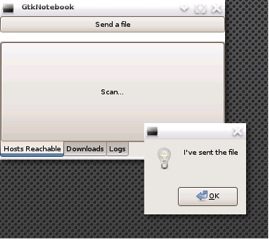
\includegraphics[width=5cm]{1.jpg} %ou image.png, .jpeg etc.
\caption{Success Notification after the sending of a file} %la légende
\label{api} %l'étiquette pour faire référence à cette image
\end{figure} %on ferme l'environnement figure

\begin{figure}[!h] %on ouvre l'environnement figure
\centering
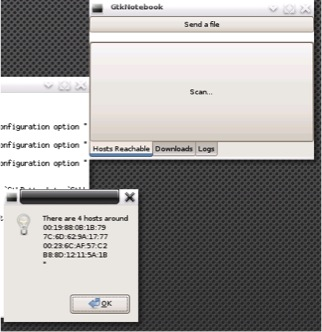
\includegraphics[width=5cm]{2.jpg} %ou image.png, .jpeg etc.
\caption{Scanning Devices PopUp} %la légende
\label{api} %l'étiquette pour faire référence à cette image
\end{figure} %on ferme l'environnement figure

\begin{figure}[!h] %on ouvre l'environnement figure
\centering
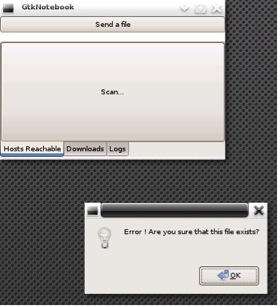
\includegraphics[width=5cm]{3.jpg} %ou image.png, .jpeg etc.
\caption{Notification Error - When the user tries to send a file that doesn't exist} %la légende
\label{api} %l'étiquette pour faire référence à cette image
\end{figure} %on ferme l'environnement figure

\begin{figure}[!h] %on ouvre l'environnement figure
\centering
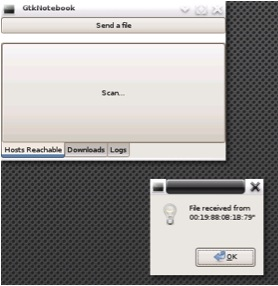
\includegraphics[width=5cm]{4.jpg} %ou image.png, .jpeg etc.
\caption{Notification for a file received} %la légende
\label{api} %l'étiquette pour faire référence à cette image
\end{figure} %on ferme l'environnement figure
 
\end{document}